\documentclass{beamer}
\usepackage{amsmath}
\usepackage{mathtools}
\usepackage{xspace}
\usepackage{centernot}
\usepackage{collectbox}
\usepackage{tikz}
\usetikzlibrary{arrows.meta,arrows,positioning,calc}
\usepackage{pgfplots}
\pgfplotsset{compat=1.5.1}
\pgfplotsset{every tick label/.append style={font=\footnotesize}}

\newcommand{\drop}[1]{#1}
%\renewcommand{\drop}[1]{}
\newcommand{\enablepause}{}
%%%; Macros
\newcommand{\bin}[2]{\mathrm{B}\parens{#1, #2}}
\DeclareMathOperator{\sgn}{sgn}
\newcommand{\idot}[2]{\parens{#1 \cdot #2}}
\newcommand{\indot}[2]{#1 \cdot #2}
\newcommand{\checkfor}[3]{%
  \ifcsname#1\endcsname%
  #2
  \else%
  #3
  \fi%
}

\setlength{\fboxsep}{5pt}%
\setlength{\fboxrule}{1pt}
% Mathbox
\makeatletter
\newcommand*\mathbox[2][black]{%
   \let\bgroup{\romannumeral-`}%
   \@Acolorboxed{#1}#2&&\ENDDNE
}
\def\@Acolorboxed#1#2&#3&#4\ENDDNE{%
  \ifnum0=`{}\fi
  \setbox\z@\hbox{$\displaystyle#2{}\m@th$\kern\fboxsep \kern\fboxrule}%
  \edef\@tempa{\kern\wd\z@ \kern-\the\wd\z@ \fboxsep\the\fboxsep \fboxrule\the\fboxrule}%
  \@tempa
  \fcolorbox{#1}{white}{\m@th$\displaystyle#2#3$}%
}
\newcommand*\mathboxx[2][black]{%
   \let\bgroup{\romannumeral-`}%
   \@Acolorboxedd{#1}#2&&\ENDDNE
}
\def\@Acolorboxedd#1#2&#3&#4\ENDDNE{%
  \ifnum0=`{}\fi
  \setbox\z@\hbox{$\displaystyle#2{}\m@th$\kern\fboxsep \kern\fboxrule}%
  \edef\@tempa{\kern\wd\z@ & \kern-\the\wd\z@ \fboxsep\the\fboxsep \fboxrule\the\fboxrule}%
  \@tempa
  \fcolorbox{#1}{white}{\m@th$\displaystyle#2#3$}%
}
\makeatother

% Autosize
\newcommand\swapifbranches[3]{#1{#3}{#2}}
\makeatletter
\MHInternalSyntaxOn
\patchcmd{\DeclarePairedDelimiter}{\@ifstar}{\swapifbranches\@ifstar}{}{}
\MHInternalSyntaxOff
\makeatother

\newcommand{\grad}{\nabla}
\DeclareMathOperator{\pers}{Per_{\sigma}}
\DeclareMathOperator{\per}{Per}
\DeclarePairedDelimiter\parens{(}{)}
\DeclarePairedDelimiter\braces{\{}{\}}
\DeclarePairedDelimiter\bracp{[}{]}
\DeclarePairedDelimiter\iproddelim{\langle}{\rangle}
\DeclarePairedDelimiter\abs{\lvert}{\rvert}
\DeclarePairedDelimiter\norm{\lVert}{\rVert}
\DeclarePairedDelimiter\floor{\lfloor}{\rfloor}
\newcommand{\iprod}[2]{\iproddelim{#1, #2}}
\newcommand{\contradiction}{\Rightarrow\!\Leftarrow}
\newcommand{\R}[1]{\mathbb{R}^{#1}}

\makeatletter
% I prefer upgamma
\let\oldgamma\gamma
\renewcommand{\gamma}{\@ifstar{\gamma}{\upgamma}}

% Better spacing by default
\let\oldexists\exists
\def\exists{\@ifstar{\oldexists}{\; \oldexists \,}}

\let\oldforall\forall
\def\forall{\@ifstar{\oldforall}{\; \oldforall \,}}
\makeatother
%%%:
%%%; Unique Macros
\newcommand{\B}[1]{\mathrm{B}\parens{#1}}
\newcommand{\G}[1]{\Gamma\parens{#1}}
\newcommand{\ks}{\kappa_\sigma}
\newcommand{\Pu}{\Pi^+}
\newcommand{\chit}[2]{\overline{\chi}_{#1}\parens{#2}}
\newcommand{\chitt}[1]{\overline{\chi}_{#1}}
\newcommand{\E}[1]{\mathcal{E}\parens{#1}}
\newcommand{\pdot}[2]{\idot{#1}{#2}}
\newcommand{\Prs}{\mathcal{P}_S}
\newcommand{\Prsbp}{\Prs b^\perp}
\newcommand{\Prsbpa}{\abs{\Prsbp}}
\newcommand{\mq}{K}
\newcommand{\C}{\mathcal{C}}
\newcommand{\pp}{\Pi^{+}}
\newcommand{\ppc}{\Pi^{+^c}}
\newcommand{\haus}[2]{\mathcal{H}^{#1}\parens{#2}}
\newcommand{\limuo}{\lim_{\sigma \uparrow 1} \,}
\newcommand{\xde}{\mathcal{X}(\partial E)}
\newcommand{\xs}{\mathcal{X}(\mathcal{S})}
\newcommand{\ms}{\mathcal{S}}
\newcommand{\mc}{\mathcal{C}}
\newcommand{\mt}{\mathcal{T}}
\newcommand{\md}{\mathcal{D}}
\newcommand{\Ae}{\mathcal{A}_e}
\newcommand{\Ai}{\mathcal{A}_i}
\DeclareMathOperator{\area}{Area}
\DeclareMathOperator{\areas}{Area_{\sigma}}
\DeclareMathOperator{\len}{Len}
\DeclareMathOperator{\lens}{Len_{\sigma}}
\newcommand{\U}[1]{\mathcal{U}_{#1}}
\newcommand{\Aodd}{\mathcal{A}^+_{\text{odd}}}
\newcommand{\Aeven}{\mathcal{A}^+_{\text{even}}}
\newcommand{\Ap}{\mathcal{A}^+}
\newcommand{\chib}[1]{\overline{\chi}_{#1}}
%%%:
%%%; Beamer Macros
\newcommand{\titleori}{\frametitle{Origins of Nonlocal Curvature of Curves}}
\checkfor{enablepause}{
  \newcommand{\pau}{\pause}
  \newcommand<>{\paumathbox}[1]{\alt#2{\mathbox[black]{#1}}{\mathbox[white]{#1}}}
}{
  \newcommand{\pau}{}
  \newcommand<>{\paumathbox}[1]{\mathbox[black]{#1}}
  \renewcommand<>{\onslide}[1]{#1}
}
\newcommand\Wider[2][3em]{%
\makebox[\linewidth][c]{%
  \begin{minipage}{\dimexpr\textwidth+#1\relax}
  \raggedright#2
  \end{minipage}%
  }%
}
\makeatletter
\newlength\beamerleftmargin
\setlength\beamerleftmargin{\Gm@lmargin}
\newlength\beamerrightmargin
\setlength\beamerrightmargin{\Gm@rmargin}
\newlength\beamertopmargin
\setlength\beamertopmargin{\Gm@rmargin}
\makeatother

\tikzset{
  invisible/.style={opacity=0},
  visible on/.style={alt=#1{}{invisible}},
  alt/.code args={<#1>#2#3}{%
    \alt<#1>{\pgfkeysalso{#2}}{\pgfkeysalso{#3}} % \pgfkeysalso doesn't change the path
  },
}
%%%:
%%%; Appearance
% Margins
\setlength{\parindent}{0pt}
\setlength{\parskip}{0in}
\setbeamersize{text margin left=5mm, text margin right=5mm}

% Actual theme declaration
\definecolor{LUCRed}{rgb}{0.58431373, 0.17254902, 0.29411765}
\usetheme{Szeged}
\usecolortheme{beaver}

% remove 2nd section from header
\makeatletter
\beamer@theme@subsectionfalse

% Allows frames to contain only subtitles
\defbeamertemplate*{frametitle}{only sub}[1][left]
{
  \ifbeamercolorempty[bg]{frametitle}{}{\nointerlineskip}%
  \@tempdima=\textwidth%
  \advance\@tempdima by\beamer@leftmargin%
  \advance\@tempdima by\beamer@rightmargin%
  \begin{beamercolorbox}[sep=0.3cm,#1,wd=\the\@tempdima]{frametitle}
    \usebeamerfont{frametitle}%
    \vbox{}\vskip-1ex%
    \if@tempswa\else\csname beamer@fte#1\endcsname\fi%
    %\strut\insertframetitle\strut\par% <-- This line is commented out
    {%
      \ifx\insertframesubtitle\@empty%
      \else%
      {\usebeamerfont{framesubtitle}\usebeamercolor[fg]{framesubtitle}\insertframesubtitle\strut\par}%
      \fi
    }%
    \vskip-1ex%
    \if@tempswa\else\vskip-.3cm\fi% set inside beamercolorbox... evil here...
  \end{beamercolorbox}%
}
\makeatother
% remove navigation buttons in bottom right
\setbeamertemplate{navigation symbols}{}

% Colors
\setbeamercolor{alerted text}{fg=LUCRed}
\setbeamercolor{titlelike}{parent=palette primary,fg=LUCRed}
\setbeamercolor{frametitle}{bg=gray!10!white}
\setbeamercolor{frametitle right}{bg=gray!60!white}
\setbeamercolor{palette primary}{bg=gray!30!white, fg=LUCRed}
\setbeamercolor{palette secondary}{bg=LUCRed, fg=white}
\setbeamercolor{palette tertiary}{bg=LUCRed, fg=white}
\setbeamercolor{palette quaternary}{bg=LUCRed, fg=white}
\setbeamercolor{structure}{fg=LUCRed}
\setbeamercolor{section in toc}{fg=LUCRed}

% LUC logo
\graphicspath{{./figures/}}
\titlegraphic{
\includegraphics[width=2cm]{luclogo}}
%%%:
%%%; Metadata
\title[Computing Limit of Nonlocal Curvature of Curves in $\R{n}$]{Computing the limit of the Nonlocal Curvature of Curves in $\R{n}$}
\author{Dan Zimmerman}
\institute{AMS 2024 Fall Eastern Sectional Meeting, Oct 19, 2024}
\date{}
%%%:

\begin{document}
\drop{
%%%; Title: Page 1
\frame{\titlepage}
%%%:
%%%; Origins: Pages 2-7
%%%; Page 2
\setbeamertemplate{frametitle}[default]
\begin{frame}
  \titleori
  Basic functional:
  $$
    J(u) = \int_{\R{n}} \abs{\grad u}^2 d V
  $$
  \pau
  Replace $\grad u$ with its fractional counterpart, with $0 < \sigma < 1$
  $$
    \grad^\sigma u(x) \simeq \int_{\R{n}} \frac{(u(y)-u(x))(y-x)}{\abs{y-x}^{n+\sigma+1}} dy
  $$
  \pau
  to obtain
  $$
    J_{\sigma}(u) = \int_{\R{n}} \abs{\grad^\sigma u}^2 d V
    \simeq \int_{\R{n}} \int_{\R{n}} \frac{\abs{u(x)-u(y)}^2}{\abs{x-y}^{n+\sigma}} d x d y
  $$
  \pau
  % Idea here: want to be a function of sets
  Consider $u = \chi_E$ for bounded $E$: $\int_E \int_{E^c} \frac{1}{\abs{x-y}^{n+\sigma}} dxdy$
  $$
    \pers(E) := \frac{1}{\alpha_{n-1}} \int_E \int_{E^c} \frac{1}{\abs{x-y}^{n+\sigma}} dx dy
  $$
\end{frame}
%%%:
%%%; Page 3
\setbeamertemplate{frametitle}[only sub]
\begin{frame}
  \titleori
  \framesubtitle{Nonlocal minimal surfaces - Caffarelli, Roquejoffre, Savin (2010)}
  \onslide<1->{
    For unbounded $E$, fix $\Omega$ bounded, and set
    \begin{align*}
      \pers(E, \Omega) &:= \frac{1}{\alpha_{n-1}} \parens{\int_{E \cap \Omega} \int_{E^c} + \int_{E \cap \Omega^c} \int_{E^c \cap \Omega}} \frac{1}{\abs{x-y}^{n+\sigma}} dx dy \\
      \onslide<2->{&= \paumathbox<3->{\raggedright \frac{1}{\alpha_{n-1}} \int_E \int_{E^c} \frac{\max\braces{ \chi_\Omega(x), \chi_\Omega(y) }}{\abs{x-y}^{n+\sigma}} dx dy}}
    \end{align*}
  }
  \onslide<4->{
    $E$ minimizer of when $\pers(E, \Omega) \le \pers(F, \Omega) \text{ s.t. } F \setminus \Omega = E \setminus \Omega$,
  }
  \onslide<5->{
    $$
    \int_{\R{n}} \frac{\chi_E(x) - \chi_{E^c}(x)}{\abs{z - x}^{n + \sigma}} dx = 0 \qquad z \in \partial E
    $$
  }
  \onslide<6->{
    Nonlocal mean curvature at $z \in \partial E$
    $$
    H_\sigma(z) := \frac{1}{\omega_{n-1}} \int_{\R{n}} \frac{\chi_E(x) - \chi_{E^c}(x)}{\abs{z-x}^{n+\sigma}} dx
    $$
  }
\end{frame}
%%%:
%%%; Page 4
\begin{frame}
  \titleori
  \framesubtitle{On the nonlocal curvatures of open surfaces - Paroni, Podio-Guidugli, Seguin (2018)}
  \vspace{-0.4cm}
  \begin{align*}
    \pers(E, \Omega) :=& \frac{1}{\alpha_{n-1}} \int_E \int_{E^c} \frac{\max\braces{\chi_\Omega(x), \chi_\Omega(y)}}{\abs{x-y}^{n+\sigma}} dx dy \\
    \onslide<2->{=& \frac{1}{2\alpha_{n-1}} \int_{\xde} \frac{\max\braces{\chi_\Omega(x), \chi_\Omega(y)}}{\abs{x - y}^{n+\sigma}} dx dy}
  \end{align*}
  \onslide<3->{
    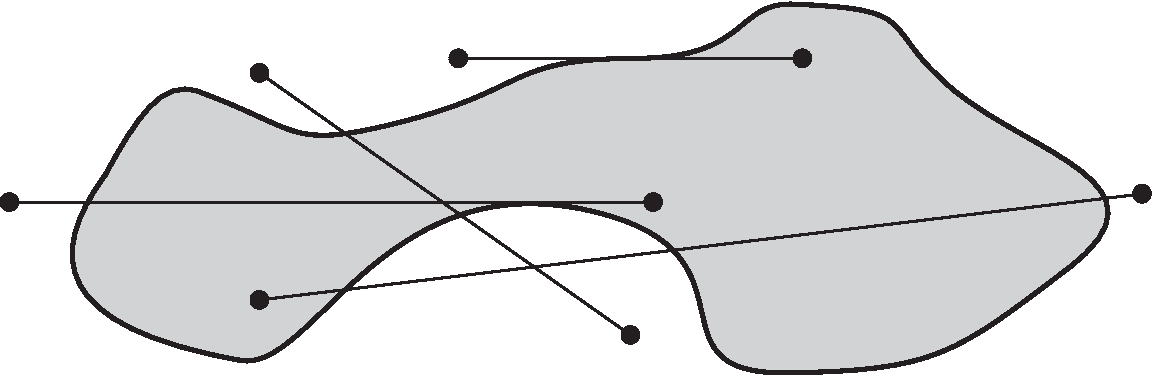
\includegraphics[width=\paperwidth-\beamerleftmargin-\beamerrightmargin]{crossings} \\
    \raggedleft \footnotesize $\xde = \braces{(x, y) \in \R{n} \times \R{n} \mid \haus{0}{[x, y] \cap \partial E} \text{ is odd}}$
  }

  \onslide<4->{
    $$
      \areas (\ms, \Omega) := \frac{1}{2 \alpha_{n-1}} \int_{\xs} \frac{\max\braces{\chi_\Omega(x), \chi_\Omega(y)}}{\abs{x-y}^{n+\sigma}} dx dy
    $$
  }
\end{frame}
%%%:
%%%; Page 5 (Drop)
%\begin{frame}
%  \titleori
%  \framesubtitle{On the nonlocal curvatures of open surfaces - Paroni, Podio-Guidugli, Seguin (2018)}
%  Minimizer $\ms$ of $\areas(\cdot, \Omega)$ with fixed boundary satisfies
%  $$
%  \parens{\int_{\Ae(z)} - \int_{\Ai(z)}} \frac{1}{\abs{z - y}^{n+\sigma}} dy = 0 \qquad z \in \ms
%  $$
%  \pau
%
%  \begin{figure}
%  \centering
%  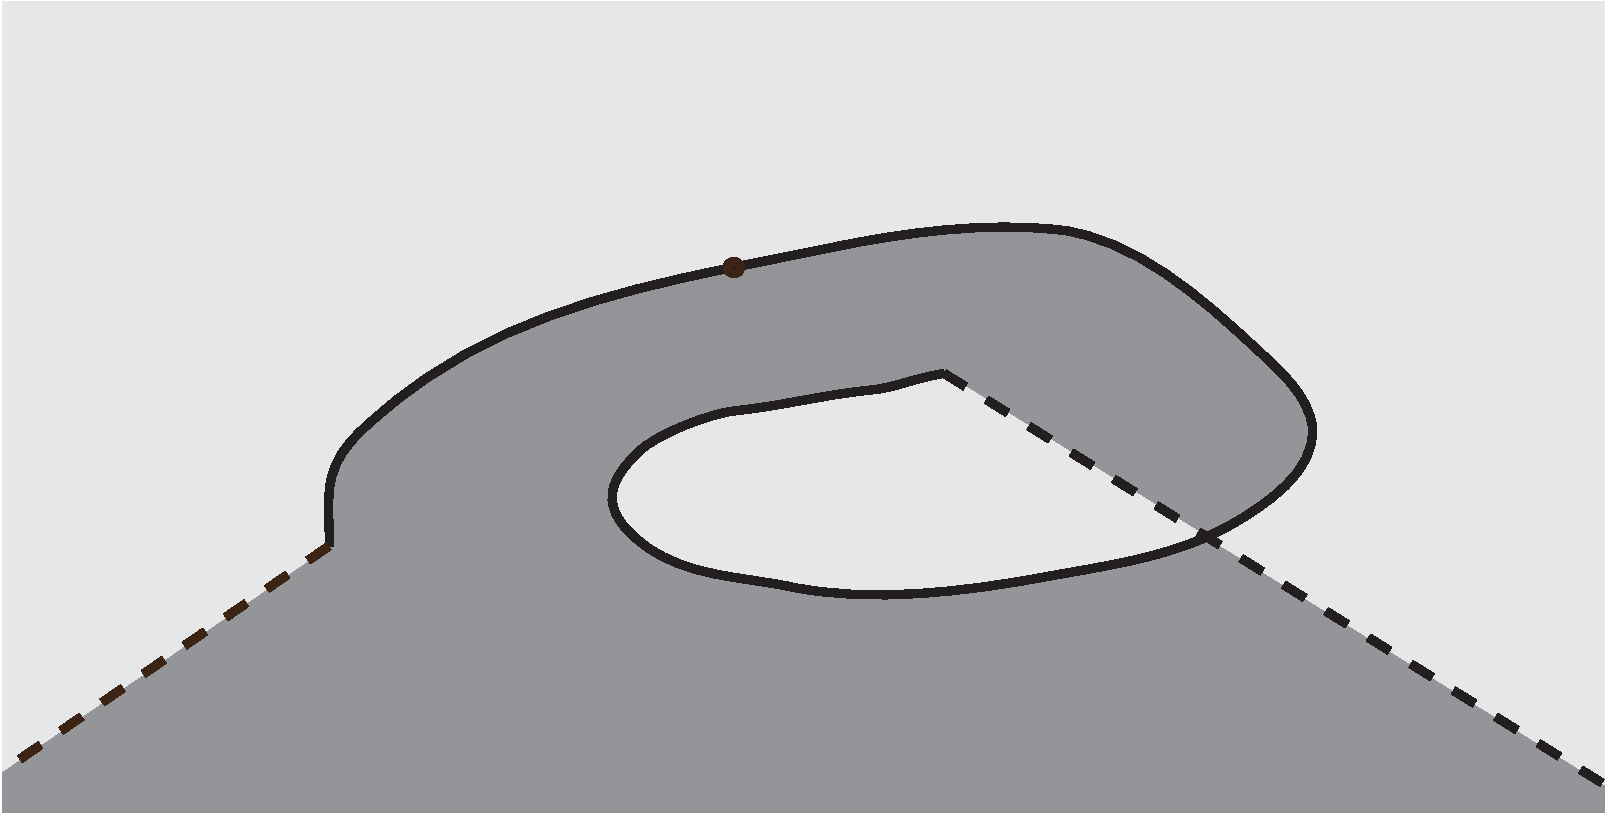
\includegraphics[width=3.5in]{aiae}
%  \thicklines
%  \put(-143,77){$z$}
%  \put(-230,90){$\Ai(z)$}
%  \put(-150,20){$\Ae(z)$}
%  \put(-135,100){$n_\ms$}
%  \put(-55,80){$\ms$}
%  \put(-152.5,92){\rotatebox[origin=c]{102}{$\vector(1,0){25}$}}
%  \put(-183,45){$n_\ms$}
%  \put(-183,45){\rotatebox[origin=c]{168}{$\vector(1,0){25}$}}
%  \end{figure}
%  %\begin{align*}
%  %  \Ae(z) &:= \{ y \in \R{n} \mid ((z, y) \in \xs, (z-y) \cdot n(z) > 0) \\
%  %  & \qquad \qquad \quad \text{ or } ((z, y) \in \xs^c, (z-y) \cdot n(z) < 0) \} \\
%  %  \Ai(z) &:= \{ y \in \R{n} \mid ((z, y) \in \xs^c, (z-y) \cdot n(z) > 0) \\
%  %  & \qquad \qquad \quad \text{ or } ((z, y) \in \xs, (z-y) \cdot n(z) < 0) \}
%  %\end{align*}
%\end{frame}
%%%:
%%%; Page 5
\begin{frame}
  \titleori
  \framesubtitle{A fractional notion of length and an associated nonlocal curvature - Seguin (2020)}
  \vspace{-5mm}
  \begin{align*}
    \area_\sigma^{(n=2)}(\ms, \Omega) &= \frac{1}{4} \int_{\xs} \frac{\max\braces{\chi_\Omega(x), \chi_\Omega(y)}}{\abs{x - y}^{2 + \sigma}} dx dy
    \onslide<2->{
      \intertext{
        Disks! (intersecting $\ms$ odd times)
        \begin{figure}
          \centering
          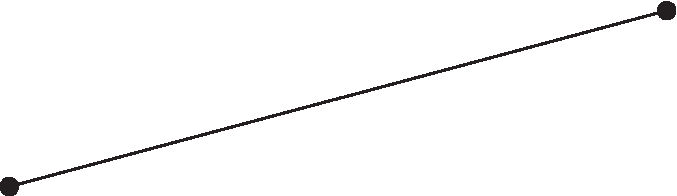
\includegraphics[width=2in]{SegDisc}
          \thicklines
          \put(-73,12){$p$}
          \put(-155,-10){$x=p-ru^\perp$}
          \put(-5,25){$y=p+ru^\perp$}
          \put(-85,30){$u$}
          \put(-60,30){$u^\perp$}
          \put(-74,18){$\bullet$}
          \put(-86.5,25){\rotatebox[origin=c]{105}{$\vector(1,0){20}$}}
          \put(-73,23.5){\rotatebox[origin=c]{15}{$\vector(1,0){20}$}}
        \end{figure}
      }
    }
    \onslide<3->{
      &= \frac{1}{2} \int_{\md(\ms)} \frac{\max\braces{\chi_\Omega(p - ru^\perp), \chi_\Omega(p + ru^\perp)}}{(2r)^{1+\sigma}} d \haus{4}{p, u, r}
    }
  \end{align*}
  \onslide<4->{
    Generalizes nicely
    $$
      \lens(\mc, \Omega) := \frac{\Gamma\parens{\frac{n+1}{2}}^2}{2\pi^{n-1}} \int_{\md(\mc)} \frac{\sup_{v \in \U{n} \cap {u}^\perp} \chi_\Omega(p + rv)}{r^{n-1+\sigma}} d \haus{2n}{p, u, r}
    $$
  }
\end{frame}
%%%:
%%%; Page 6
\begin{frame}
  \titleori
  \framesubtitle{A fractional notion of length and an associated nonlocal curvature - Seguin (2020)}
  Minimizing over $\mc$ with fixed boundary, $z \in \mc$
  $$
  \parens{\int_{\Aeven(z)} - \int_{\Aodd(z)}} \frac{\parens{a \cdot t(z)}b - \parens{b \cdot t(z)}a}{r^{1+\sigma}} d\haus{2n-2}{a, b, r} = 0
  $$
  \pau
  \begin{figure}
  \centering
  \thicklines
  \scalebox{.75}{
    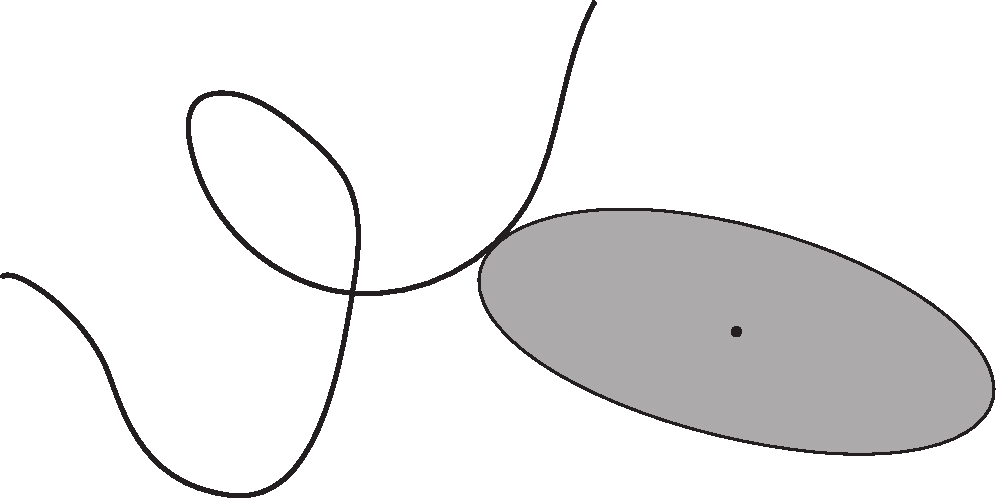
\includegraphics[height=4cm]{cb2}
    \put(-123,61){$z$}
    \put(-117,56){$\bullet$}
    \put(-70,25){$z+ra$}
    \put(-180,25){$\mc$}
    \put(-113,45){$a$}
    \put(-113,54){\rotatebox[origin=c]{-20}{$\vector(1,0){20}$}}
    \put(-50,48){$b$}
    \put(-69,44){\rotatebox[origin=c]{75}{$\vector(1,0){20}$}}
  }
  \end{figure}
  \pau
  Nonlocal {\it vector} curvature
  $$
  \kappa_\sigma(z) := \parens{\int_{\Aodd(z)} - \int_{\Aeven(z)}} \frac{\parens{a \cdot t(z)}b - \parens{b \cdot t(z)}a}{r^{1+\sigma}} d\haus{2n-2}{a, b, r}
  $$
\end{frame}
%%%:
%%%; Page 7
\begin{frame}
  \titleori
  \framesubtitle{Asymptotics of fractional \& Nonlocal Quantities}
  \onslide<2->{
    \begin{align*}
      \limuo (1-\sigma) \pers(E, B_r) &= \per(E, B_r) \\
      \limuo (1 - \sigma) H_\sigma(z) &= H(z) \\
      \onslide<3->{\limuo (1 - \sigma) \lens(\mc, \Omega) &= \len(\mc, \Omega) \\}
      \onslide<4->{
        \mathboxx[black]{\limuo (1 - \sigma) \onslide<5->{\; ? \;} \kappa_\sigma(z) &\stackrel{?}{=} \kappa(z)}
      }
    \end{align*}
  }
\end{frame}
%%%:
%%%:
%%%; Project: 8-14
%%%; Page 8 (Outline)
\setbeamertemplate{frametitle}[default]
\begin{frame}
  \frametitle{Argument Outline}
  \begin{enumerate}
    \item<1-> For $\C_R$ circle with radius $R$, in $\R{2}$
      $$
        \limuo (1 - \sigma) \onslide<2->{\frac{1}{\mq_2}} \kappa_\sigma(z) = \kappa(z) \quad z \in \C_R \onslide<2->{,\, \mq_2 \in \R{}}
      $$
    \item<3-> Use (1), same $\C_R$, in $\R{n}$
      $$
        \limuo (1 - \sigma) \onslide<4->{\frac{1}{\mq(n)}} \kappa_\sigma(z) = \kappa(z) \quad z \in \C_R \onslide<4->{, \, \mq(n) \in \R{} \text{ s.t. } \mq(2) = \mq_2}
      $$
    \item<5-> For arbitrary $\mc$ and $\C_R$ ($R=1/\kappa(z; \C))$ at $z \in \mc$
      $$
        \limuo (1-\sigma) \abs{\kappa_\sigma(z; \C) - \kappa_\sigma(z; \C_R)} = 0
      $$
    \item<6-> Combine 2 \& 3, show for arbitrary $\mc$, $z \in \mc$
      \begin{align*}
        \mathbox[LUCRed]{\limuo (1 - \sigma) \frac{1}{\mq(n)} \kappa_\sigma(z) = \kappa(z)}
      \end{align*}
  \end{enumerate}
\end{frame}
%%%:
%%%; Page 9
\setbeamertemplate{frametitle}[default]
\begin{frame}
  \frametitle{$z \in \C_R$, $n=2$}
  $$
    \kappa_\sigma = \parens{\int_{\Aeven(z)} - \int_{\Aodd(z)}} \frac{\parens{a \cdot t}b - \parens{b \cdot t}a}{r^{1+\sigma}} d\haus{2}{a, b, r}
  $$
  \onslide<2->{
    $\R{2} = \mathrm{span}\braces{t, n}$
    \onslide<3->{
      \begin{align*}
        \indot{\kappa_\sigma}{t} &= \parens{\int_{\Aeven(z)} - \int_{\Aodd(z)}} \frac{\idot{a}{t}\idot{b}{t} - \idot{b}{t}\idot{a}{t}}{r^{1+\sigma}} d\haus{2}{a, b, r} = 0 \\
        \onslide<4->{
          \indot{\kappa_\sigma}{n} &= \parens{\int_{\Aeven(z)} - \int_{\Aodd(z)}} \frac{\idot{a}{t}\idot{b}{n} - \idot{b}{t}\idot{a}{n}}{r^{1+\sigma}} d\haus{2}{a, b, r} \\
          \onslide<5->{&= \int_{\Ap(z)} \chit{\Aeven(z)}{a,b,r} \frac{\idot{a}{t}\idot{b}{n} - \idot{b}{t}\idot{a}{n}}{r^{1+\sigma}} d\haus{2}{a, b, r}}
        }
      \end{align*}
      \onslide<5->{
        \raggedleft $\footnotesize \chitt{\Aeven(z)} = \chi_{\Aeven(z)} - \chi_{\parens{\Aeven(z)}^c} = \chi_{\Aeven(z)} - \chi_{\Aodd(z)}$
      }
    }
  }
\end{frame}
%%%:
%%%; Page 10
\setbeamertemplate{frametitle}[only sub]
\begin{frame}
  \frametitle{.}
  \framesubtitle{$z \in \C_R$, $n=2$}
  \vspace{-4ex}
  \begin{align*}
    \onslide<2->{\indot{b}{t} > 0 \implies b &= \sgn \idot{a}{n} a^\perp} \\
    \onslide<3->{\text{Disks: } u &:= 2ra}
  \end{align*}
%;
\begin{center}
  \makebox[0pt]{
\begin{tikzpicture}
\begin{axis}[ 
    axis lines = none,
    ticks = none,
    axis line style={-},
    ymin=-1.25, ymax=-0.35,
    xmin=-1.5, xmax=1.5,
    axis equal image,
    width={\paperwidth+\beamerleftmargin+\beamerrightmargin}
]

\draw[color=white, fill = blue, opacity=0.2] (axis cs:-15, -13) rectangle (axis cs:15, 1);
\draw[color=white, fill = green, opacity=0.6] (axis cs:-15, -13) rectangle (axis cs:15, -1);
\draw[color=white, fill = red, opacity=0.6] (axis cs:-15, -13) rectangle (axis cs:15, -1);

\def\figphi{30}
%p/4-phi/2=theta where phi is angle from x-axis of unit circle to top right point of triangle
\def\figtheta{45-\figphi/2}

%\draw[color=black] (axis cs:-1, -1) -- (axis cs:1, -1);
  \addplot[data cs=polar, green, opacity=0.6, domain=0:180,samples=180,smooth, fill=green, fill opacity=0.6, shift={(0, {transformdirectiony(-1)})}] (x, {2*cos(90 - x)});
  \addplot[data cs=polar, red, opacity=0.6, domain=0:180,samples=180,smooth, fill=red, fill opacity=0.6, shift={(0, {transformdirectiony(-1)})}] (x, {cos(90 - x)});
  \node at (axis cs:-0.98, -0.4) {$\C_R$};
  \node[visible on=<4-5>] at (axis cs:-0.25, -0.5) {$\Aeven$};
  \node[visible on=<4-5>] at (axis cs:-0.7, -1.15) {$\Aeven$};
  \node[visible on=<5>] at (axis cs:-0.65, -0.45) {$\Aodd$};
  \node[visible on=<5>] at (axis cs:-1.2, -0.45) {$\Aodd$};
  \node[visible on=<6->] at (axis cs:0.65, -0.45) {$\pp$};
  \node[visible on=<6->] at (axis cs:0.7, -1.15) {$\pp$};
  \node[visible on=<6->] at (axis cs:1.2, -0.45) {$\ppc$};
\begin{scope}[shift={(0, {transformdirectiony(-1)})}]
  %\node[label={225:{\footnotesize $0$}},circle,fill,inner sep=2pt] at (axis cs:0,0) {};
  %\draw (axis cs:0.25,0) arc(0:{\figtheta}:{transformdirectionx(0.25)});
  %\node at (axis cs:{0.17*cos(0.5*\figtheta)}, {0.17*sin(0.5*\figtheta)}) {$\theta$};
  %\draw (axis cs:0,0) -- (axis cs:{1.1*2*sin(\figtheta)*cos(\figtheta)},{1.1*2*sin(\figtheta)*sin(\figtheta)}) -- (axis cs:0, 1);
  \draw [decorate,decoration={brace,amplitude=10pt}] (axis cs:0,0) -- (axis cs:{(1.1/2)*2*sin(\figtheta)*cos(\figtheta)},{(1.1/2)*2*sin(\figtheta)*sin(\figtheta)}) node [black,midway,yshift={transformdirectiony(0.1)}, xshift={transformdirectionx(-0.1)}] {\footnotesize $r$};
  %\draw [decorate,decoration={brace,amplitude=15pt, mirror}] (axis cs:0,0) -- (axis cs:{(1.1)*2*sin(\figtheta)*cos(\figtheta)},{(1.1)*2*sin(\figtheta)*sin(\figtheta)}) node [black,midway,yshift={transformdirectiony(-0.15)}, xshift={transformdirectionx(0.15)}] {\footnotesize $u$};
  \draw [visible on=<3->,-Latex,thick] (axis cs:0,0) -- (axis cs:{(1.1)*2*sin(\figtheta)*cos(\figtheta)},{(1.1)*2*sin(\figtheta)*sin(\figtheta)}) node [black,yshift={transformdirectiony(-0.1)}, xshift={transformdirectionx(0)}] {\footnotesize $u$};
\end{scope}


%\draw [decorate,decoration={brace,amplitude=10pt,mirror}] (axis cs:-0.01,-0.01) -- (axis cs:-0.01,{-1+0.01}) node [black,midway,xshift={transformdirectionx(-0.15)}] {\footnotesize $R$};

%\draw [decorate,decoration={brace,amplitude=5pt}] (axis cs:0,-1) -- (axis cs:{0.5*cos(\figphi)},{0.5*(-sin(\figphi)-1)}) node [black,midway, xshift={transformdirectionx(-0.07)}, yshift={transformdirectiony(0.07)}] {\footnotesize $l$};

\draw [-Latex, thick] (axis cs:0,-1) -- (axis cs:{0.3*cos(\figtheta)},{0.3*sin(\figtheta)-1}) node [black, xshift={transformdirectionx(0.03)}, yshift={transformdirectiony(-0.03)}] {\footnotesize $a$};
\draw [-Latex, thick] (axis cs:0, -1) -- (axis cs:0.3, -1) node [black,xshift={transformdirectionx(0)},yshift={transformdirectiony(-0.06)}] {\footnotesize $t$};
\draw [-Latex, thick] (axis cs:0, -1) -- (axis cs:0, -0.7) node [black,xshift={transformdirectionx(0.05)},yshift={transformdirectiony(0)}] {\footnotesize $n$};
\draw (axis cs:0,0) circle [radius=1];

  %\node[label={{$-1$}}] at (axis cs:-0.5,0.5) {};
  %\node[label={{$-1$}}] at (axis cs:-0.5,-1.2) {};
  %\node[label={{$+1$}}] at (axis cs:-0.3,-0.7) {};

\end{axis}
\end{tikzpicture}
}
\end{center}
%:
\onslide<6->{
  \begin{align*}
    \displaystyle \pp :=& \braces{ u \in \R{2} \mid \idot{u}{n} < 0 \text{ or } \frac{\abs{u}}{2} < R\idot{\frac{u}{\abs{u}}}{n} } \\
    \onslide<7->{
      \indot{\kappa_\sigma}{n} =& -2^{\sigma + 1/2} \int_{\R{2}} \frac{\chit{\pp}{u}\sgn\idot{u}{n}}{\abs{u}^{2+\sigma}} d\haus{2}{u} \\
    }
  \end{align*}
}
%  \onslide<4->{
%$$
%  \indot{\kappa_\sigma}{n} = \int_{\Ap} \frac{\parens{\chi_{\Aeven} - \chi_{\Aodd}}\sgn\idot{a}{n}}{r^{1+\sigma}} d\haus{2}{a,b,r}
%$$
%}
\end{frame}
%%%:
%%%; Page 11
\begin{frame}
  \frametitle{.}
  \framesubtitle{$z \in \C_R$, $n=2$}
  \vspace{-5mm}
  \begin{align*}
    \indot{\kappa_\sigma}{n} &= -2^{\sigma + 1/2} \paumathbox<3->{\int_{\R{2}} \frac{\chit{\pp}{u}\sgn\idot{u}{n}}{\abs{u}^{2+\sigma}} d\haus{2}{u}} \\
    \onslide<2->{
      &=-2^{\sigma + 1/2} \paumathbox<3->{
        \frac{-2^{1 - \sigma}}{\sigma R^\sigma} \bin{\frac{1}{2}}{\frac{1-\sigma}{2}}
      } \\
    }
    \onslide<4->{
      \limuo \parens{1-\sigma} \idot{\kappa_\sigma}{n} &= 
      2^{3/2} \paumathbox<5->{\limuo \frac{\parens{1-\sigma}}{\sigma R^\sigma} \B{\frac{1}{2}, \frac{1-\sigma}{2}}} \\
      %\frac{\G{\frac{1}{2}}\G{\frac{1-\sigma}{2}}}{\G{1-\frac{\sigma}{2}}} \\
      \onslide<6->{
        &= \frac{2^{3/2}\sqrt{\pi}}{R} \limuo \parens{1-\sigma} \G{\frac{1-\sigma}{2}} 
        \onslide<7->{
          = \paumathbox<8->{
            \alt<9>{\overbrace{2^{5/2}\sqrt{\pi}}^{K_2} \overbrace{\frac{1}{R}}^{\kappa}}{2^{5/2}\sqrt{\pi} \frac{1}{R}}
          }
        }
      }
    }
  \end{align*}
\end{frame}
%%%:
%%%; Page 12
\setbeamertemplate{frametitle}[default]
\begin{frame}
  \frametitle{$z \in \C_R$, $n \ge 2$}
  \vspace{-5mm}
  $$
    \kappa_\sigma(z) := \parens{\int_{\Aeven(z)} - \int_{\Aodd(z)}} \frac{\parens{a \cdot t(z)}b - \parens{b \cdot t(z)}a}{r^{1+\sigma}} d\haus{2n-2}{a, b, r}
  $$
  \begin{enumerate}
    \item<2-> Slice on intersection with $t \times n$ plane (i.e. $u$ in $2$d)
    \item<3-> Recognize $\indot{\kappa_\sigma}{n}$ is only non-zero component
      \begin{enumerate}
        \item<4->[Conjecture] Any curve in $k$ dimensional subspace only depends on $k$-dimensional curvature
      \end{enumerate}
    \item<5-> Slice on $r$, i.e. group disks with common $u$ with common $r$
    \item<6-> Some more coarea applications, recognition of spheres \& beta functions...
    \onslide<7->{
      \begin{align*}
      \indot{
        \kappa_\sigma
      }{n} =
        -&2^{\sigma-3/2}\omega_{n-3}^2 \B{\frac{3}{2}, \frac{n-2}{2}} \B{\frac{\sigma+2}{2}, \frac{n-2}{2}} \\
        \onslide<7-9>{
          &\paumathbox<8-9>{
            \alt<7-8>{
              \int_{\R{2}} \frac{\chit{\Pu}{u} \sgn{\idot{n}{u}}}{\abs{u}^{2+\sigma}} \, d\haus{2}{u}
            }{
              \frac{-2^{1 - \sigma}}{\sigma R^\sigma} \bin{\frac{1}{2}}{\frac{1-\sigma}{2}}
            }
          }
        }
      \end{align*}
    }
  \end{enumerate}
\end{frame}
%%%:
%%%; Page 13
\setbeamertemplate{frametitle}[only sub]
\begin{frame}
  \frametitle{.}
  \framesubtitle{$z \in \C_R$, $n \ge 2$}
  \begin{align*}
    \limuo & \parens{1-\sigma}\idot{\kappa_\sigma}{n} \\
    &= 
    \frac{\omega_{n-3}^2}{\sqrt{2}} \B{\frac{3}{2}, \frac{n-2}{2}} \B{\frac{\sigma+2}{2}, \frac{n-2}{2}} \paumathbox<2->{\frac{\parens{1-\sigma}}{\sigma R^\sigma} \bin{\frac{1}{2}}{\frac{1-\sigma}{2}}} \\
    \onslide<3->{
      &= 
        \alt<4>{
          \overbrace{\omega_{n-3}^2 \sqrt{2\pi} \B{\frac{3}{2}, \frac{n-2}{2}} \B{\frac{\sigma+2}{2}, \frac{n-2}{2}}}^{K(n)} \overbrace{\frac{1}{R}}^{\kappa}
        }{
          \omega_{n-3}^2 \sqrt{2\pi} \B{\frac{3}{2}, \frac{n-2}{2}} \B{\frac{\sigma+2}{2}, \frac{n-2}{2}} \frac{1}{R}
        }
    }
  \end{align*}
\end{frame}
%%%:
}
%%%; Page 14
\setbeamertemplate{frametitle}[default]
\begin{frame}
  \frametitle{$2$nd order approximation}
  Want $\limuo (1-\sigma) \abs{\kappa_\sigma(z; \C) - \kappa_\sigma(z; \C_R)} = 0$ for arbitrary $\C$, $\C_{R=1/\kappa}$
  \onslide<2->{
    \begin{align*}
      \abs{\kappa_\sigma(z; \C) - \kappa_\sigma(z; \C_R)} &\lesssim \int_{\Ap} \frac{\abs{\chitt{\Aeven(\C)} - \chitt{\Aeven(\C_R)}}}{r^{1+\sigma}}
    \end{align*}
  }
  %; Ribbon figure
  \onslide<3->{
    \begin{center}
      \vspace{-15mm}
      \makebox[0pt]{
        \begin{tikzpicture}
          \node [
            above right,
            inner sep=0
          ] (image) at (0, 0) {
            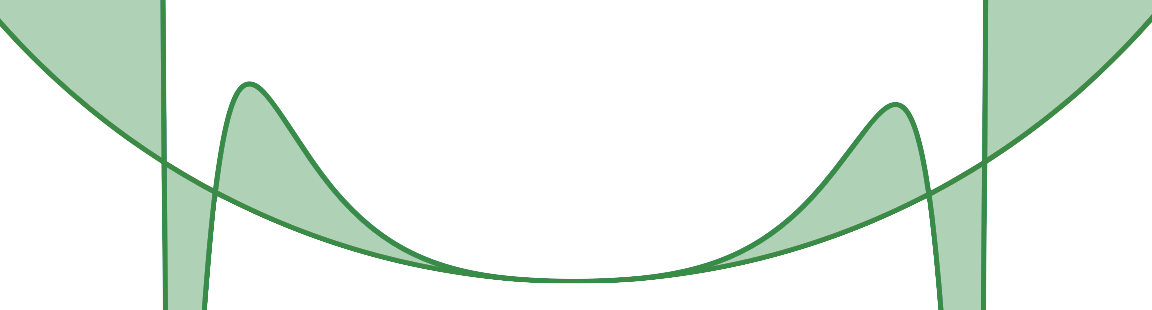
\includegraphics[width=\paperwidth]{ribbon}
          };
          \begin{scope}[
            x={($0.1*(image.south east)$)},
            y={($0.1*(image.north west)$)},
          ]
            %\draw[black,step=1] (image.south west) grid (image.north east);
            \draw (7.75, 7.2) node [black] {$\C$};
            \draw (9.7, 7) node [black] {$\C_R$};
            \draw [visible on=<4->,-Latex,thick] (5,1) -- (6,9) node [black] {};
            \draw [visible on=<4->,-Latex,thick] (5,1) -- (3,0) node [black] {};
            \draw [visible on=<5->,-Latex,thick] (5,1) -- (8.25,6) node [black] {};
            \draw [visible on=<5->,-Latex,thick] (5,1) -- (8.9,3) node [black] {};
            \draw [visible on=<6->,-Latex,thick] (5,1) -- (7.3,3) node [black] {};
            \draw [visible on=<6->,-Latex,thick] (5,1) -- (1.6,3) node [black] {};
            \draw [visible on=<7->,-Latex,thick] (5,1) -- (1.89,8) node [black] {};
            \draw [visible on=<7->,-Latex,thick] (5,1) -- (1.87,3.87) node [black] {};
          \end{scope}
        \end{tikzpicture}
      }
    \end{center}
  }
  %:
  \begin{itemize}
    \item<8->[C1] Disks whose boundary intersects ribbon are all that matter
    \item<9->[C2] With the right area \& coarea applications the integral over relevant disks vanishes
  \end{itemize}
  % we believe we can use arguements from intersection from differential topology to show this
\end{frame}
%%%:
%%%; Page 15
\setbeamertemplate{frametitle}[default]
\begin{frame}
  \frametitle{Final Result}
  Arbitrary $\C$, $K(n) = \omega_{n-3}^2 \sqrt{2\pi} \B{\frac{3}{2}, \frac{n-2}{2}} \B{\frac{\sigma+2}{2}, \frac{n-2}{2}}$, $z \in \C$
  $$
    \mathbox[LUCRed]{\limuo \parens{1-\sigma} \frac{1}{K(n)} \kappa_\sigma(z) = \kappa(z)}
  $$
  \pau
  New definition?
  $$
    \hspace{-2mm}
    \kappa_\sigma(z) := \frac{1}{K(n)} \parens{\int_{\Aeven(z)} - \int_{\Aodd(z)}} \frac{\parens{a \cdot t(z)}b - \parens{b \cdot t(z)}a}{r^{1+\sigma}} d\haus{2n-2}{a, b, r}
  $$
\end{frame}
%%%:
%%%:
%%%; Fin: Page 16
\begin{frame}
  \begin{center}
    \Huge Fin
  \end{center}
\end{frame}
%%%:

\end{document}
